\documentclass[10pt]{article}
\usepackage[margin=0.78in]{geometry}
\usepackage[T1]{fontenc}
\usepackage{lmodern}
\usepackage{microtype}
\usepackage{graphicx}
\usepackage{booktabs}
\usepackage{placeins}
\usepackage{xcolor}
\usepackage{hyperref}
\definecolor{navy}{HTML}{16324F}
\definecolor{teal}{HTML}{087E8B}
\hypersetup{colorlinks=true,linkcolor=navy,urlcolor=teal}
\title{\textcolor{navy}{When Should IDM-Viz Refit?}\\[3pt]\large A Label-Safe Schedule Audit}
\author{23I-2581 and 23I-2604\\Data Analysis and Visualization --- Phase 3 addendum}
\date{17 November 2026}
\begin{document}\maketitle
\begin{abstract}
This controlled extension compares a frozen logistic classifier with periodic, global released-error-triggered, and region-local released-error-triggered refitting. It tests whether the triggers avoid unnecessary stationary-stream updates and whether schedules recover accuracy after a synthetic conditional reversal. Thirty paired seeds, three label delays, and two synthetic mechanisms are used. This remains a bounded synthetic policy comparison, not a claim of operational benefit.
\end{abstract}
\section{Protocol}
The stream contains 96 batches of 500 observations. A single logistic classifier is trained on the frozen historical set; its scaler and a three-region MiniBatchKMeans partition are fit on training rows. The periodic policy refits at forecast clocks 25, 49, and 73. The global trigger requires both latest released cohorts to exceed calibration error by 0.10. The local trigger requires two eligible released cohorts in one frozen region to exceed that region's calibration error by 0.10; each cohort needs at least 20 rows and each calibration region needs at least 20 rows. Both triggers have an eight-clock cooldown and a three-update cap. A global update uses historical training rows plus at most 2,000 recent released labels. A local update uses only that region's historical training rows and at most 2,000 recent released labels from that region; other regions retain the global frozen fallback. Thresholds and regions are fixed without monitoring outcomes.

For delay $d$, source batch $s$ is available before forecast batch $b$ only when $s+d<b$. The current batch is predicted before its labels can be released. The detector uses stored predictions only after the scheduled release. The primary unit for uncertainty is the seed: batch metrics are aggregated within each seed, then a paired seed bootstrap forms 95\% intervals.

\section{Results}
\begin{figure}[ht]
\centering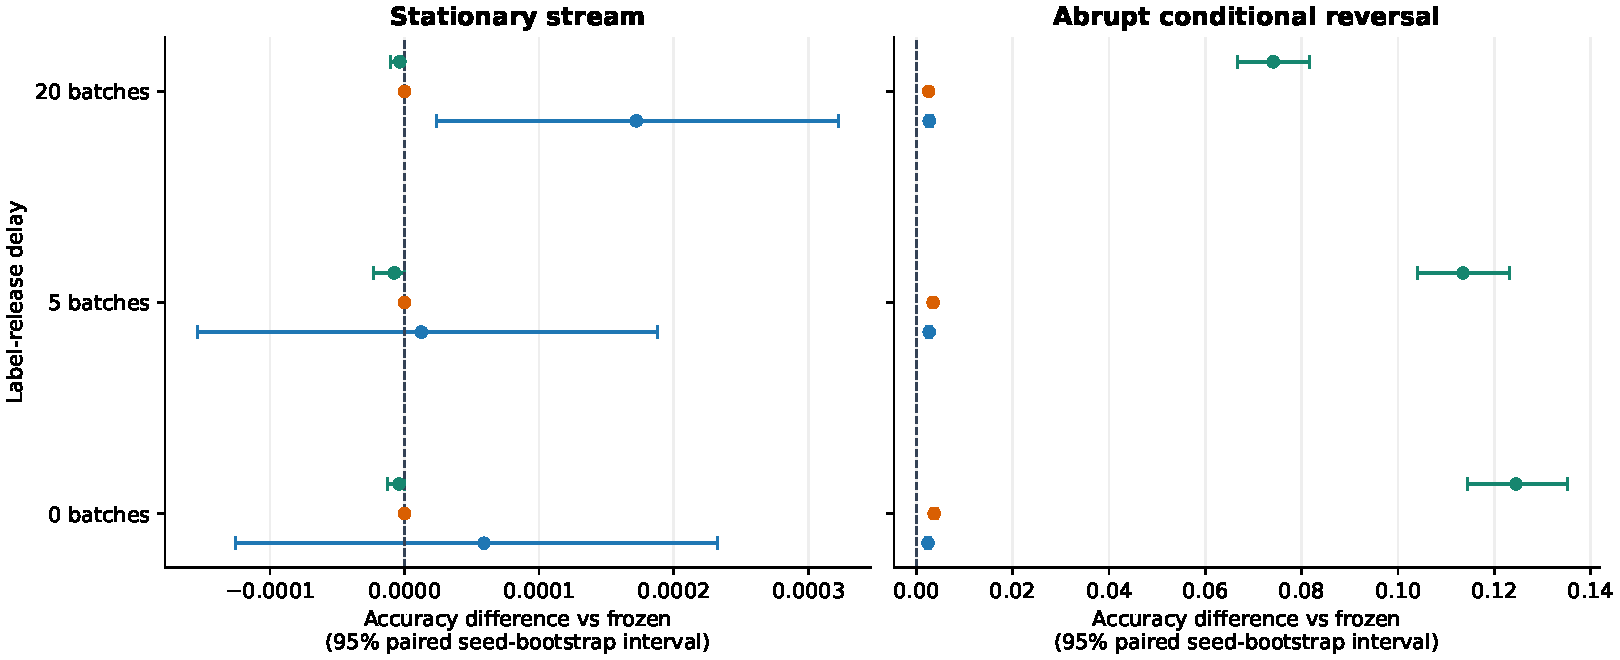
\includegraphics[width=\linewidth]{adaptation_schedule.pdf}
\caption{Paired accuracy differences from the frozen policy; blue denotes periodic refitting, orange global trigger, and green region-local trigger. Intervals resample the 30 matched seeds.}
\end{figure}
\begin{table}[ht]
\centering\small
\begin{tabular}{@{}llrrrrrr@{}}
\toprule
Mechanism & Delay & Frozen & Periodic & Global & Local & Global updates & Local updates\\
\midrule
Stationary & 0 & 0.724 & 0.725 & 0.724 & 0.724 & 0.00 & 0.03\\
Stationary & 5 & 0.724 & 0.724 & 0.724 & 0.724 & 0.00 & 0.03\\
Stationary & 20 & 0.724 & 0.725 & 0.724 & 0.724 & 0.00 & 0.03\\
Reversal & 0 & 0.388 & 0.390 & 0.391 & 0.512 & 3.00 & 3.00\\
Reversal & 5 & 0.388 & 0.390 & 0.391 & 0.501 & 3.00 & 3.00\\
Reversal & 20 & 0.388 & 0.390 & 0.390 & 0.462 & 3.00 & 3.00\\
\bottomrule
\end{tabular}
\caption{Mean accuracy across paired seeds; trigger updates are averaged across seeds.}
\end{table}

For abrupt reversal, the local trigger improved all-stream mean accuracy over frozen by 12.45 percentage points at zero delay (paired 95\% seed-bootstrap interval 11.45--13.51 points), 11.35 points at five-batch delay (10.42--12.32), and 7.41 points at twenty-batch delay (6.68--8.17). The global trigger gains were 0.37, 0.35, and 0.26 points, respectively. Local gains are substantial in this generator, but this is a single synthetic reversal design with a fixed training-fitted partition and trigger; it does not establish general superiority or transfer. Under stationarity, one of 30 seeds triggered one local update (at all three delays); paired accuracy differences were effectively zero. The global trigger did not update. Read \texttt{paired\_accuracy\_differences.csv} for all estimates and paired intervals.

\FloatBarrier
\section{Interpretation and limits}
This extension evaluates one global and one frozen-region local trigger, but does not cover alternative thresholds, region counts, multiple classifiers, multiple real-world streams, concept-change recovery guarantees, or equal consumed-label budgets against frozen prediction. The local policy uses a training-fitted unsupervised partition and can leave a region on its global fallback when evidence is sparse or a local refit lacks both classes. Fit-row counts are a computational proxy, not wall-clock or energy measurements. Synthetic reversal results cannot establish utility for deployment.

\section{Reproduction}
Run from the workspace root:
\begin{verbatim}
powershell -NoProfile -ExecutionPolicy Bypass \\
  -File .\\scripts\\reproduce_adaptation_schedule_audit.ps1
\end{verbatim}
The runner receipt records code/configuration and output hashes, label-release semantics, seed bank and software versions. Contract tests check that no forecast consumes same-clock labels and that the result tables contain all locked seed-policy cells.

\end{document}
